\documentclass[]{article}
\usepackage{lmodern}
\usepackage{amssymb,amsmath}
\usepackage{ifxetex,ifluatex}
\usepackage{fixltx2e} % provides \textsubscript
\ifnum 0\ifxetex 1\fi\ifluatex 1\fi=0 % if pdftex
  \usepackage[T1]{fontenc}
  \usepackage[utf8]{inputenc}
\else % if luatex or xelatex
  \ifxetex
    \usepackage{mathspec}
  \else
    \usepackage{fontspec}
  \fi
  \defaultfontfeatures{Ligatures=TeX,Scale=MatchLowercase}
\fi
% use upquote if available, for straight quotes in verbatim environments
\IfFileExists{upquote.sty}{\usepackage{upquote}}{}
% use microtype if available
\IfFileExists{microtype.sty}{%
\usepackage{microtype}
\UseMicrotypeSet[protrusion]{basicmath} % disable protrusion for tt fonts
}{}
\usepackage[margin=1in]{geometry}
\usepackage{hyperref}
\hypersetup{unicode=true,
            pdfborder={0 0 0},
            breaklinks=true}
\urlstyle{same}  % don't use monospace font for urls
\usepackage{color}
\usepackage{fancyvrb}
\newcommand{\VerbBar}{|}
\newcommand{\VERB}{\Verb[commandchars=\\\{\}]}
\DefineVerbatimEnvironment{Highlighting}{Verbatim}{commandchars=\\\{\}}
% Add ',fontsize=\small' for more characters per line
\usepackage{framed}
\definecolor{shadecolor}{RGB}{248,248,248}
\newenvironment{Shaded}{\begin{snugshade}}{\end{snugshade}}
\newcommand{\KeywordTok}[1]{\textcolor[rgb]{0.13,0.29,0.53}{\textbf{#1}}}
\newcommand{\DataTypeTok}[1]{\textcolor[rgb]{0.13,0.29,0.53}{#1}}
\newcommand{\DecValTok}[1]{\textcolor[rgb]{0.00,0.00,0.81}{#1}}
\newcommand{\BaseNTok}[1]{\textcolor[rgb]{0.00,0.00,0.81}{#1}}
\newcommand{\FloatTok}[1]{\textcolor[rgb]{0.00,0.00,0.81}{#1}}
\newcommand{\ConstantTok}[1]{\textcolor[rgb]{0.00,0.00,0.00}{#1}}
\newcommand{\CharTok}[1]{\textcolor[rgb]{0.31,0.60,0.02}{#1}}
\newcommand{\SpecialCharTok}[1]{\textcolor[rgb]{0.00,0.00,0.00}{#1}}
\newcommand{\StringTok}[1]{\textcolor[rgb]{0.31,0.60,0.02}{#1}}
\newcommand{\VerbatimStringTok}[1]{\textcolor[rgb]{0.31,0.60,0.02}{#1}}
\newcommand{\SpecialStringTok}[1]{\textcolor[rgb]{0.31,0.60,0.02}{#1}}
\newcommand{\ImportTok}[1]{#1}
\newcommand{\CommentTok}[1]{\textcolor[rgb]{0.56,0.35,0.01}{\textit{#1}}}
\newcommand{\DocumentationTok}[1]{\textcolor[rgb]{0.56,0.35,0.01}{\textbf{\textit{#1}}}}
\newcommand{\AnnotationTok}[1]{\textcolor[rgb]{0.56,0.35,0.01}{\textbf{\textit{#1}}}}
\newcommand{\CommentVarTok}[1]{\textcolor[rgb]{0.56,0.35,0.01}{\textbf{\textit{#1}}}}
\newcommand{\OtherTok}[1]{\textcolor[rgb]{0.56,0.35,0.01}{#1}}
\newcommand{\FunctionTok}[1]{\textcolor[rgb]{0.00,0.00,0.00}{#1}}
\newcommand{\VariableTok}[1]{\textcolor[rgb]{0.00,0.00,0.00}{#1}}
\newcommand{\ControlFlowTok}[1]{\textcolor[rgb]{0.13,0.29,0.53}{\textbf{#1}}}
\newcommand{\OperatorTok}[1]{\textcolor[rgb]{0.81,0.36,0.00}{\textbf{#1}}}
\newcommand{\BuiltInTok}[1]{#1}
\newcommand{\ExtensionTok}[1]{#1}
\newcommand{\PreprocessorTok}[1]{\textcolor[rgb]{0.56,0.35,0.01}{\textit{#1}}}
\newcommand{\AttributeTok}[1]{\textcolor[rgb]{0.77,0.63,0.00}{#1}}
\newcommand{\RegionMarkerTok}[1]{#1}
\newcommand{\InformationTok}[1]{\textcolor[rgb]{0.56,0.35,0.01}{\textbf{\textit{#1}}}}
\newcommand{\WarningTok}[1]{\textcolor[rgb]{0.56,0.35,0.01}{\textbf{\textit{#1}}}}
\newcommand{\AlertTok}[1]{\textcolor[rgb]{0.94,0.16,0.16}{#1}}
\newcommand{\ErrorTok}[1]{\textcolor[rgb]{0.64,0.00,0.00}{\textbf{#1}}}
\newcommand{\NormalTok}[1]{#1}
\usepackage{graphicx,grffile}
\makeatletter
\def\maxwidth{\ifdim\Gin@nat@width>\linewidth\linewidth\else\Gin@nat@width\fi}
\def\maxheight{\ifdim\Gin@nat@height>\textheight\textheight\else\Gin@nat@height\fi}
\makeatother
% Scale images if necessary, so that they will not overflow the page
% margins by default, and it is still possible to overwrite the defaults
% using explicit options in \includegraphics[width, height, ...]{}
\setkeys{Gin}{width=\maxwidth,height=\maxheight,keepaspectratio}
\IfFileExists{parskip.sty}{%
\usepackage{parskip}
}{% else
\setlength{\parindent}{0pt}
\setlength{\parskip}{6pt plus 2pt minus 1pt}
}
\setlength{\emergencystretch}{3em}  % prevent overfull lines
\providecommand{\tightlist}{%
  \setlength{\itemsep}{0pt}\setlength{\parskip}{0pt}}
\setcounter{secnumdepth}{0}
% Redefines (sub)paragraphs to behave more like sections
\ifx\paragraph\undefined\else
\let\oldparagraph\paragraph
\renewcommand{\paragraph}[1]{\oldparagraph{#1}\mbox{}}
\fi
\ifx\subparagraph\undefined\else
\let\oldsubparagraph\subparagraph
\renewcommand{\subparagraph}[1]{\oldsubparagraph{#1}\mbox{}}
\fi

%%% Use protect on footnotes to avoid problems with footnotes in titles
\let\rmarkdownfootnote\footnote%
\def\footnote{\protect\rmarkdownfootnote}

%%% Change title format to be more compact
\usepackage{titling}

% Create subtitle command for use in maketitle
\newcommand{\subtitle}[1]{
  \posttitle{
    \begin{center}\large#1\end{center}
    }
}

\setlength{\droptitle}{-2em}

  \title{}
    \pretitle{\vspace{\droptitle}}
  \posttitle{}
    \author{}
    \preauthor{}\postauthor{}
    \date{}
    \predate{}\postdate{}
  

\begin{document}

\subsection{Example of Power in Repeated Measures
ANOVA}\label{example-of-power-in-repeated-measures-anova}

In a repeated measures design multiple observations are collected from
the same participants. Here, we will examine a repeated measures
experiment with 3 within-subject conditions, to illustrate how a
repeated measures ANOVA extends a dependent \emph{t}-test with 3 groups.

In the example for a two-group within design we provided a specific
formula for the sample size benefit for two groups. The sample size
needed in within-designs (NW) with more than 2 conditions, relative to
the sample needed in between-designs (NB), assuming normal distributions
and compound symmetry, and ignoring the difference in degrees of freedom
between the two types of tests, is (from Maxwell \& Delaney, 2004,
p.~562, formula 47):

\(N_{W}=\frac{N_{B}(1-\rho)}{a}\)

Where a is the number of within-subject levels.

\subsection{The relation between Cohen's f and Cohen's
d}\label{the-relation-between-cohens-f-and-cohens-d}

Whereas in the case of a repeated measures ANOVA with 2 groups we could
explain the principles of a power analysis by comparing our test against
a \emph{t}-test and Cohen's d, this becomes more difficult when we have
more than 2 groups. It is more useful to explain how to directly
calculate Cohen's f, the effect size used in power analyses for ANOVA.
Cohen's f is calculated following Cohen, 1988, formula 8.2.1 and 8.2.2:

\(f = \sqrt{\frac{\frac{\sum(\mu-\overline{\mu})^2)}N}\sigma}\)

Imagine we have a within-subject experiment with 3 conditions. We ask
people what they mood is when their alarm clock wakes them up, when they
wake up naturally on a week day, and when they wake up naturally on a
weekend day. Based on pilot data, we expect the means (on a 7 point
validated mood scale) are 3.8, 4.2, and 4.3. The standard deviation is
0.9, and the correlation between the dependent measurements is 0.7. We
can calculate Cohen's f for the ANOVA, and Cohen's dz for the contrasts:

\begin{Shaded}
\begin{Highlighting}[]
\NormalTok{mu <-}\StringTok{ }\KeywordTok{c}\NormalTok{(}\FloatTok{3.8}\NormalTok{, }\FloatTok{4.2}\NormalTok{, }\FloatTok{4.3}\NormalTok{)}
\NormalTok{sd <-}\StringTok{ }\FloatTok{0.9}
\NormalTok{f <-}\StringTok{ }\KeywordTok{sqrt}\NormalTok{(}\KeywordTok{sum}\NormalTok{((mu}\OperatorTok{-}\KeywordTok{mean}\NormalTok{(mu))}\OperatorTok{^}\DecValTok{2}\NormalTok{)}\OperatorTok{/}\KeywordTok{length}\NormalTok{(mu))}\OperatorTok{/}\NormalTok{sd }\CommentTok{#Cohen, 1988, formula 8.2.1 and 8.2.2}
\NormalTok{f}
\end{Highlighting}
\end{Shaded}

\begin{verbatim}
## [1] 0.2400274
\end{verbatim}

\begin{Shaded}
\begin{Highlighting}[]
\NormalTok{r <-}\StringTok{ }\FloatTok{0.7}
\NormalTok{(}\FloatTok{4.2-3.8}\NormalTok{)}\OperatorTok{/}\FloatTok{0.9}\OperatorTok{/}\KeywordTok{sqrt}\NormalTok{(}\DecValTok{2}\OperatorTok{*}\NormalTok{(}\DecValTok{1}\OperatorTok{-}\NormalTok{r))}
\end{Highlighting}
\end{Shaded}

\begin{verbatim}
## [1] 0.5737753
\end{verbatim}

\begin{Shaded}
\begin{Highlighting}[]
\NormalTok{(}\FloatTok{4.3-3.8}\NormalTok{)}\OperatorTok{/}\FloatTok{0.9}\OperatorTok{/}\KeywordTok{sqrt}\NormalTok{(}\DecValTok{2}\OperatorTok{*}\NormalTok{(}\DecValTok{1}\OperatorTok{-}\NormalTok{r))}
\end{Highlighting}
\end{Shaded}

\begin{verbatim}
## [1] 0.7172191
\end{verbatim}

\begin{Shaded}
\begin{Highlighting}[]
\NormalTok{(}\FloatTok{4.3-4.2}\NormalTok{)}\OperatorTok{/}\FloatTok{0.9}\OperatorTok{/}\KeywordTok{sqrt}\NormalTok{(}\DecValTok{2}\OperatorTok{*}\NormalTok{(}\DecValTok{1}\OperatorTok{-}\NormalTok{r))}
\end{Highlighting}
\end{Shaded}

\begin{verbatim}
## [1] 0.1434438
\end{verbatim}

The relation between Cohen's d or dz and Cohen's f becomes more
difficult when there are multiple groups, because the relationship
depends on the pattern of the means. Cohen (1988) presents calculations
for three patterns, minimal variability (for example, for 5 means:
-0.25, 0, 0, 0, 0.25), medium variability (for example, for 5 means:
-0.25, -0.25, 0.25, 0.25, 0.25 or -0.25, -0.25, -0.25, 0.25, 0.25). For
these three patterns, formula's are available that compute Cohen's f
from Cohen's d, where d is the effect size calculated for the difference
between the largest and smallest mean (if the largest mean is 0.25 and
the smallest mean is -0.25, 0.25 - -0.25 = 0.5, so d is 0.5 divided by
the standard deviation of 0.9). In our example, d would be (4.3-3.8)/0.9
= 0.5555556. If we divide this value by sqrt(2*(1-r)) we have dz =
0.5555556/0.7745967 = 0.7172191.

I have created a custom function that will calculate f from d, based on
a specification of one of the three patterns of means. Our pattern is
most similar (but not identical) to a maximum variability pattern (two
means are high, one is lower). So we could attempt to calculate f from d
(0.5555556), by calculating d from the largest and smallest mean:

\begin{Shaded}
\begin{Highlighting}[]
\KeywordTok{source}\NormalTok{(}\StringTok{"https://raw.githubusercontent.com/Lakens/ANOVA_power_simulation/master/calc_f_d_eta.R"}\NormalTok{)}

\NormalTok{res <-}\StringTok{ }\KeywordTok{calc_f_d_eta}\NormalTok{(}\DataTypeTok{mu =}\NormalTok{ mu, }\DataTypeTok{sd =}\NormalTok{ sd, }\DataTypeTok{variability =} \StringTok{"maximum"}\NormalTok{)}
\NormalTok{res}\OperatorTok{$}\NormalTok{f}
\end{Highlighting}
\end{Shaded}

\begin{verbatim}
## [1] 0.2618914
\end{verbatim}

\begin{Shaded}
\begin{Highlighting}[]
\NormalTok{res}\OperatorTok{$}\NormalTok{d}
\end{Highlighting}
\end{Shaded}

\begin{verbatim}
## [1] 0.5555556
\end{verbatim}

We see the Cohen's f value is 0.2618914 and d = 0.5555556. The Cohen's f
is not perfectly accurate - it is assuming the pattern of means is 3.8,
4.3, 4.3, and not 3.8, 4.2, 4.3. If the means and sd is known, it is
best to calculate Cohen's f directly from these values.

\subsection{Three within conditions, medium effect
size}\label{three-within-conditions-medium-effect-size}

We can perform power analyses for within designs using simuations. We
set groups to 3 for the simulation, n = 20, and the correlation between
dependent variables to 0.8. If the true effect size is f = 0.25, and the
alpha level is 0.05, the power is 96.6\%.

In this case, we simulate data with means -0.3061862, 0.0000000, and
0.3061862, and set the sd to 1.

\begin{Shaded}
\begin{Highlighting}[]
\NormalTok{K <-}\StringTok{ }\DecValTok{3}
\NormalTok{n <-}\StringTok{ }\DecValTok{20}
\NormalTok{sd <-}\StringTok{ }\DecValTok{1}
\NormalTok{r <-}\StringTok{ }\FloatTok{0.8}
\NormalTok{alpha =}\StringTok{ }\FloatTok{0.05}
\NormalTok{f <-}\StringTok{ }\FloatTok{0.25}
\NormalTok{f2 <-}\StringTok{ }\NormalTok{f}\OperatorTok{^}\DecValTok{2}
\NormalTok{ES <-}\StringTok{ }\NormalTok{f2}\OperatorTok{/}\NormalTok{(f2}\OperatorTok{+}\DecValTok{1}\NormalTok{)}
\NormalTok{ES}
\end{Highlighting}
\end{Shaded}

\begin{verbatim}
## [1] 0.05882353
\end{verbatim}

\begin{Shaded}
\begin{Highlighting}[]
\NormalTok{mu <-}\StringTok{ }\KeywordTok{mu_from_ES}\NormalTok{(}\DataTypeTok{K =}\NormalTok{ K, }\DataTypeTok{ES =}\NormalTok{ ES)}
\KeywordTok{sqrt}\NormalTok{(}\KeywordTok{sum}\NormalTok{((mu}\OperatorTok{-}\KeywordTok{mean}\NormalTok{(mu))}\OperatorTok{^}\DecValTok{2}\NormalTok{)}\OperatorTok{/}\KeywordTok{length}\NormalTok{(mu))}\OperatorTok{/}\NormalTok{sd }\CommentTok{#Cohen, 1988, formula 8.2.1 and 8.2.2}
\end{Highlighting}
\end{Shaded}

\begin{verbatim}
## [1] 0.25
\end{verbatim}

\begin{Shaded}
\begin{Highlighting}[]
\NormalTok{string =}\StringTok{ }\KeywordTok{paste}\NormalTok{(K,}\StringTok{"w"}\NormalTok{,}\DataTypeTok{sep=}\StringTok{""}\NormalTok{)}
\NormalTok{labelnames <-}\StringTok{ }\KeywordTok{c}\NormalTok{(}\StringTok{"speed"}\NormalTok{, }\StringTok{"fast"}\NormalTok{, }\StringTok{"medium"}\NormalTok{, }\StringTok{"slow"}\NormalTok{)}

\NormalTok{design_result <-}\StringTok{ }\KeywordTok{ANOVA_design}\NormalTok{(}\DataTypeTok{string =}\NormalTok{ string,}
                   \DataTypeTok{n =}\NormalTok{ n, }
                   \DataTypeTok{mu =}\NormalTok{ mu, }
                   \DataTypeTok{sd =}\NormalTok{ sd, }
                   \DataTypeTok{r =}\NormalTok{ r, }
                   \DataTypeTok{labelnames =}\NormalTok{ labelnames)}
\end{Highlighting}
\end{Shaded}

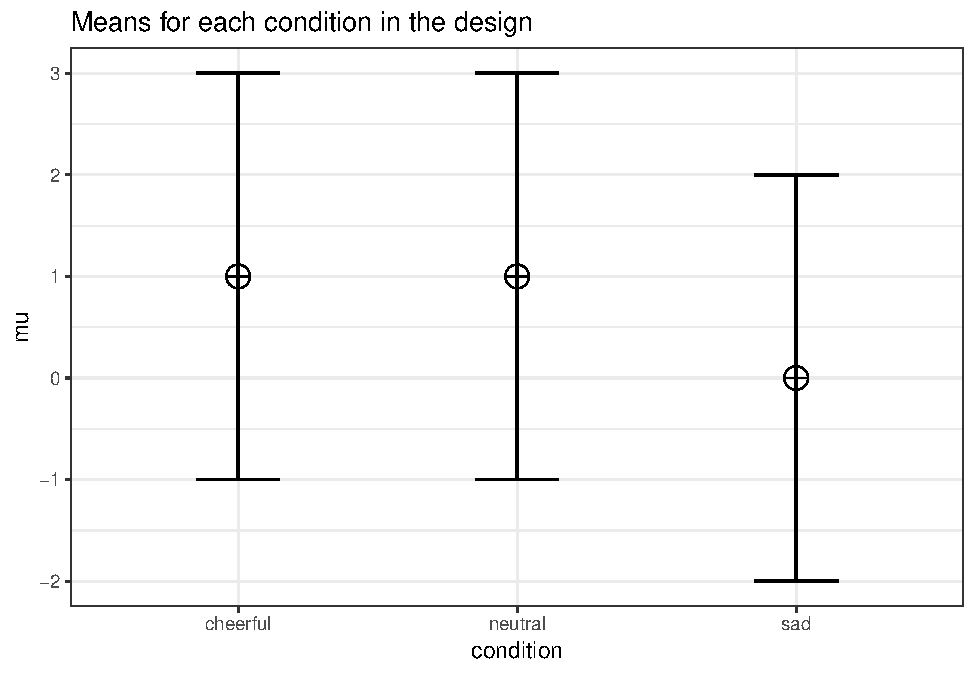
\includegraphics{2.2_validation_power_within_3x1_files/figure-latex/unnamed-chunk-3-1.pdf}

\begin{Shaded}
\begin{Highlighting}[]
\NormalTok{alpha_level <-}\StringTok{ }\FloatTok{0.05}

\KeywordTok{ANOVA_power}\NormalTok{(design_result, }\DataTypeTok{nsims =}\NormalTok{ nsims)}
\end{Highlighting}
\end{Shaded}

\begin{verbatim}
## Power and Effect sizes for ANOVA tests
##              power effect size
## anova_speed 96.529      0.3457
## 
## Power and Effect sizes for contrasts
##                            power effect size
## p_speed_fast_speed_medium 53.768      0.5035
## p_speed_fast_speed_slow   98.388      1.0084
## p_speed_medium_speed_slow 54.065      0.5058
\end{verbatim}

The results of the simulation are indeed very close to 96.9\%. We can
see this is in line with the power estimate from Gpower:

\begin{figure}
\centering
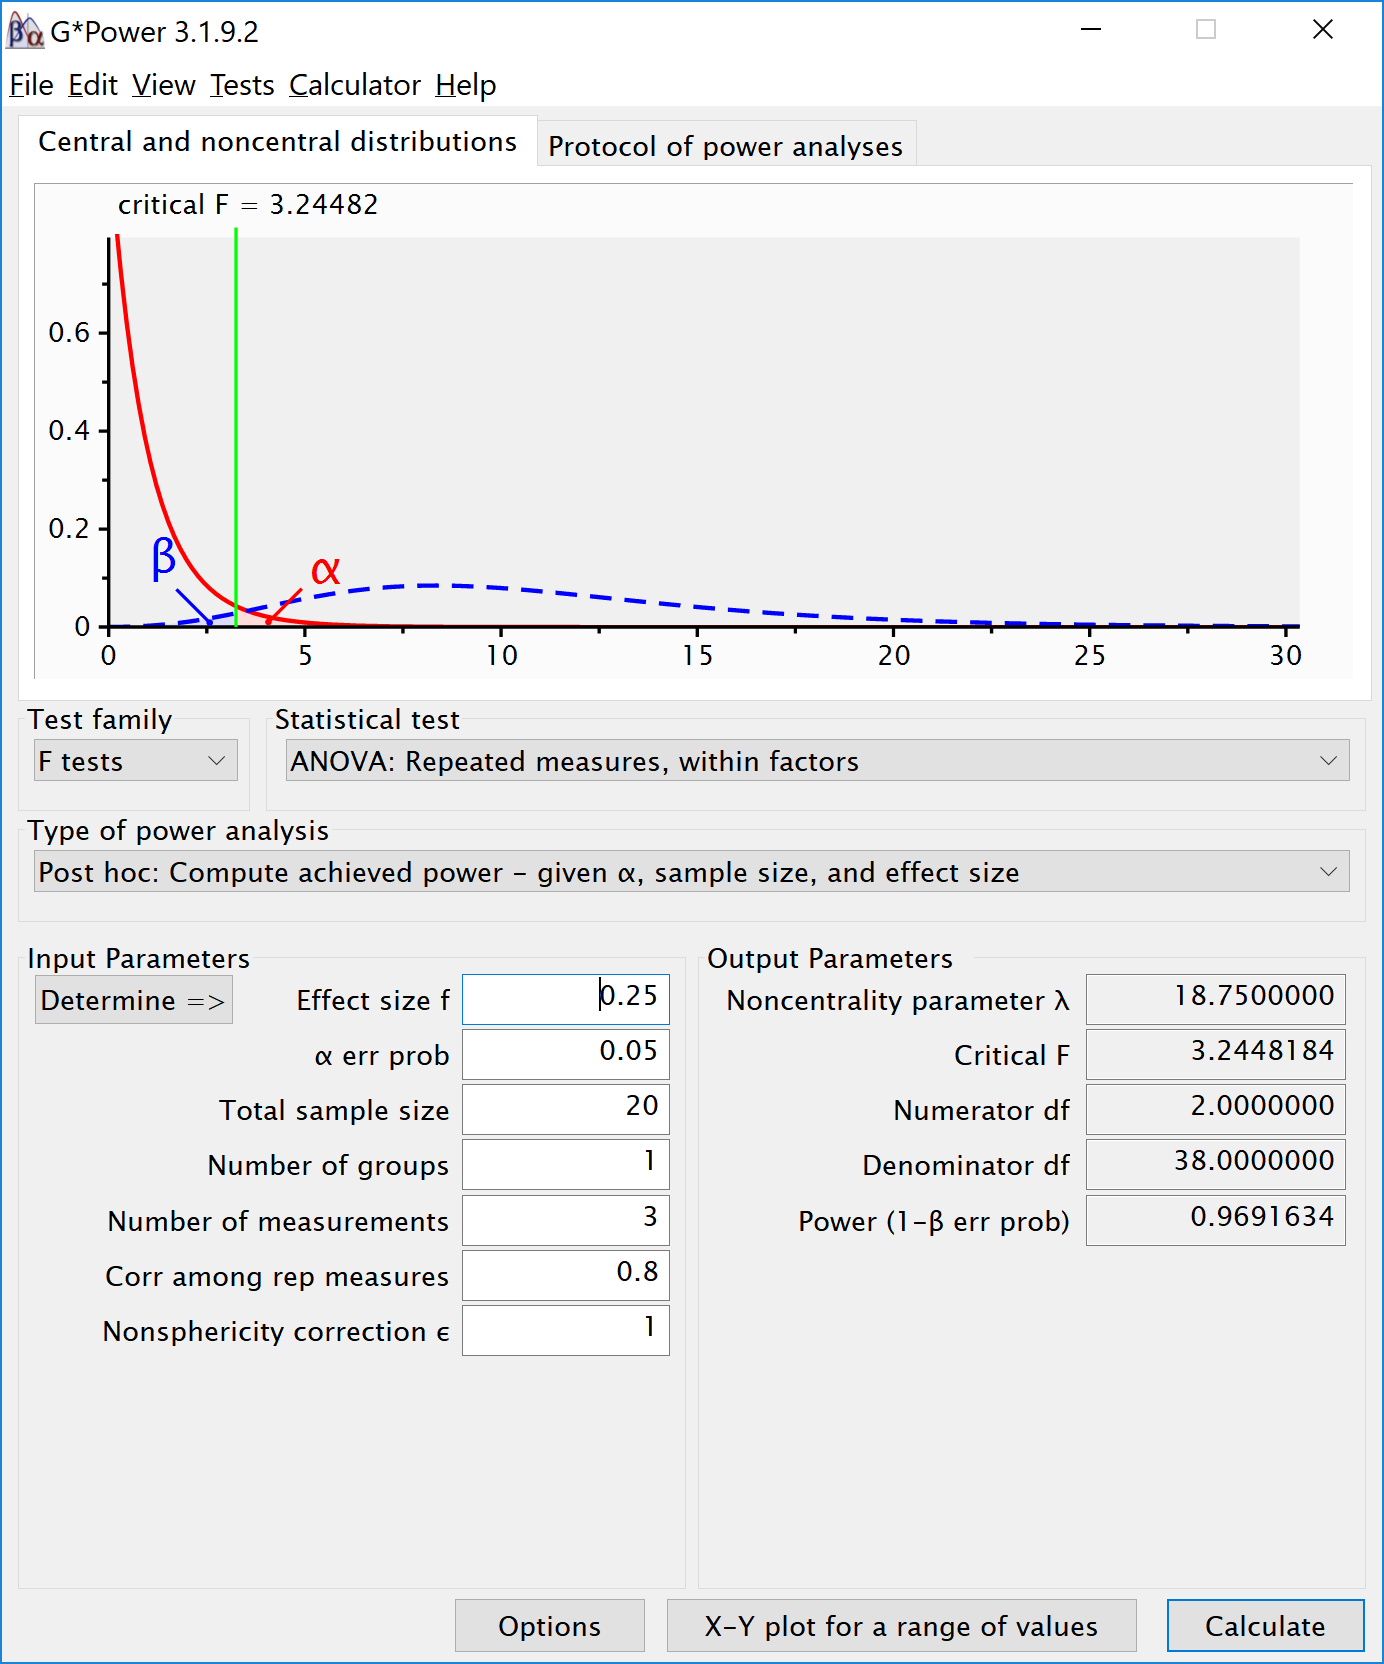
\includegraphics{screenshots/gpower_12.png}
\caption{}
\end{figure}

We can also validate this by creating the code to do a power analysis in
R from scratch:

\begin{Shaded}
\begin{Highlighting}[]
\NormalTok{K <-}\StringTok{ }\DecValTok{3} \CommentTok{#three groups}
\NormalTok{n <-}\StringTok{ }\DecValTok{20}
\NormalTok{sd <-}\StringTok{ }\DecValTok{1}
\NormalTok{r <-}\StringTok{ }\FloatTok{0.8}
\NormalTok{alpha =}\StringTok{ }\FloatTok{0.05}
\NormalTok{f <-}\StringTok{ }\FloatTok{0.25}
\NormalTok{f2 <-}\StringTok{ }\NormalTok{f}\OperatorTok{^}\DecValTok{2}
\NormalTok{ES <-}\StringTok{ }\NormalTok{f2}\OperatorTok{/}\NormalTok{(f2}\OperatorTok{+}\DecValTok{1}\NormalTok{)}
\NormalTok{ES}
\end{Highlighting}
\end{Shaded}

\begin{verbatim}
## [1] 0.05882353
\end{verbatim}

\begin{Shaded}
\begin{Highlighting}[]
\NormalTok{mu <-}\StringTok{ }\KeywordTok{mu_from_ES}\NormalTok{(}\DataTypeTok{K =}\NormalTok{ K, }\DataTypeTok{ES =}\NormalTok{ ES)}
\NormalTok{string =}\StringTok{ }\KeywordTok{paste}\NormalTok{(K,}\StringTok{"w"}\NormalTok{,}\DataTypeTok{sep=}\StringTok{""}\NormalTok{)}
\NormalTok{labelnames <-}\StringTok{ }\KeywordTok{c}\NormalTok{(}\StringTok{"speed"}\NormalTok{, }\StringTok{"fast"}\NormalTok{, }\StringTok{"medium"}\NormalTok{, }\StringTok{"slow"}\NormalTok{)}

\NormalTok{design_result <-}\StringTok{ }\KeywordTok{ANOVA_design}\NormalTok{(}\DataTypeTok{string =}\NormalTok{ string,}
                   \DataTypeTok{n =}\NormalTok{ n, }
                   \DataTypeTok{mu =}\NormalTok{ mu, }
                   \DataTypeTok{sd =}\NormalTok{ sd, }
                   \DataTypeTok{r =}\NormalTok{ r, }
                   \DataTypeTok{labelnames =}\NormalTok{ labelnames)}
\end{Highlighting}
\end{Shaded}

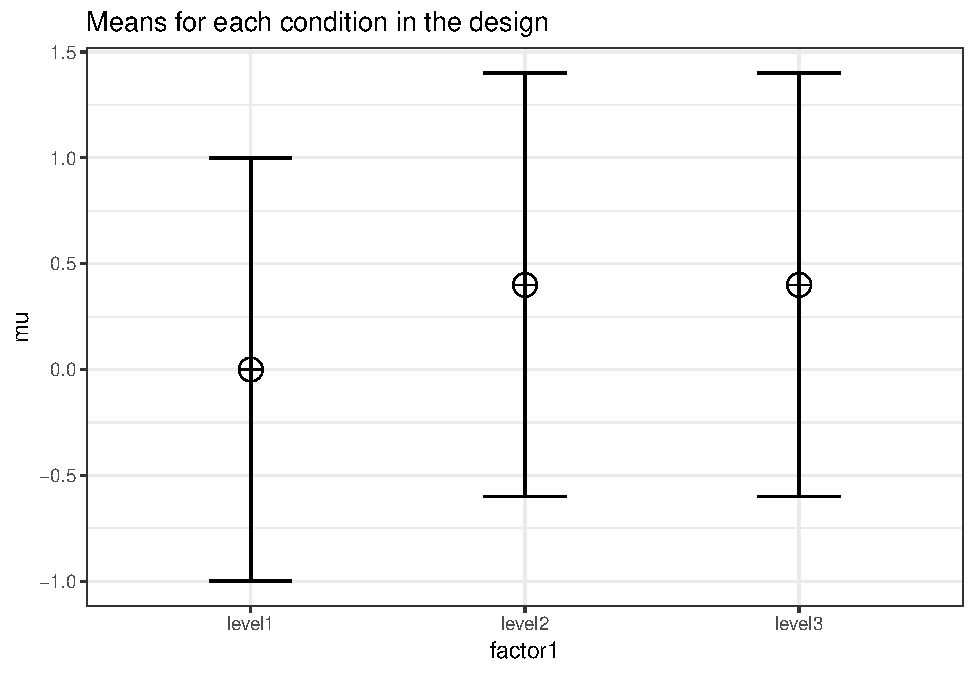
\includegraphics{2.2_validation_power_within_3x1_files/figure-latex/unnamed-chunk-4-1.pdf}

\begin{Shaded}
\begin{Highlighting}[]
\KeywordTok{power_oneway_within}\NormalTok{(design_result)}\OperatorTok{$}\NormalTok{power}
\end{Highlighting}
\end{Shaded}

\begin{verbatim}
## [1] 0.9691634
\end{verbatim}

\begin{Shaded}
\begin{Highlighting}[]
\KeywordTok{power_oneway_within}\NormalTok{(design_result)}\OperatorTok{$}\NormalTok{eta_p_}\DecValTok{2}
\end{Highlighting}
\end{Shaded}

\begin{verbatim}
## [1] 0.05882353
\end{verbatim}

\begin{Shaded}
\begin{Highlighting}[]
\KeywordTok{power_oneway_within}\NormalTok{(design_result)}\OperatorTok{$}\NormalTok{eta_p_}\DecValTok{2}\NormalTok{_SPSS}
\end{Highlighting}
\end{Shaded}

\begin{verbatim}
## [1] 0.3303965
\end{verbatim}

\begin{Shaded}
\begin{Highlighting}[]
\KeywordTok{power_oneway_within}\NormalTok{(design_result)}\OperatorTok{$}\NormalTok{Cohen_f}
\end{Highlighting}
\end{Shaded}

\begin{verbatim}
## [1] 0.25
\end{verbatim}

\begin{Shaded}
\begin{Highlighting}[]
\KeywordTok{power_oneway_within}\NormalTok{(design_result)}\OperatorTok{$}\NormalTok{Cohen_f_SPSS}
\end{Highlighting}
\end{Shaded}

\begin{verbatim}
## [1] 0.7024394
\end{verbatim}

We can even check the calculation of Cohen's f SPSS style in GPower. We
take the GPower settings as illustrated above. We click the `Options'
button, and check the radiobutton next to `As in SPSS'. Click ok, and
you will notice that the `Corr among rep measures' field has
disappeared. The correlation does not need to be entered seperately, but
is incorporated in Cohen's f. The value of Cohen's f, which was 0.25,
has changed into 0.7024394. This is the SPSS equivalent. The value is
much larger. This value, and it's corresponding partial eta-squared,
incorporate the correlation between observations.

\begin{figure}
\centering
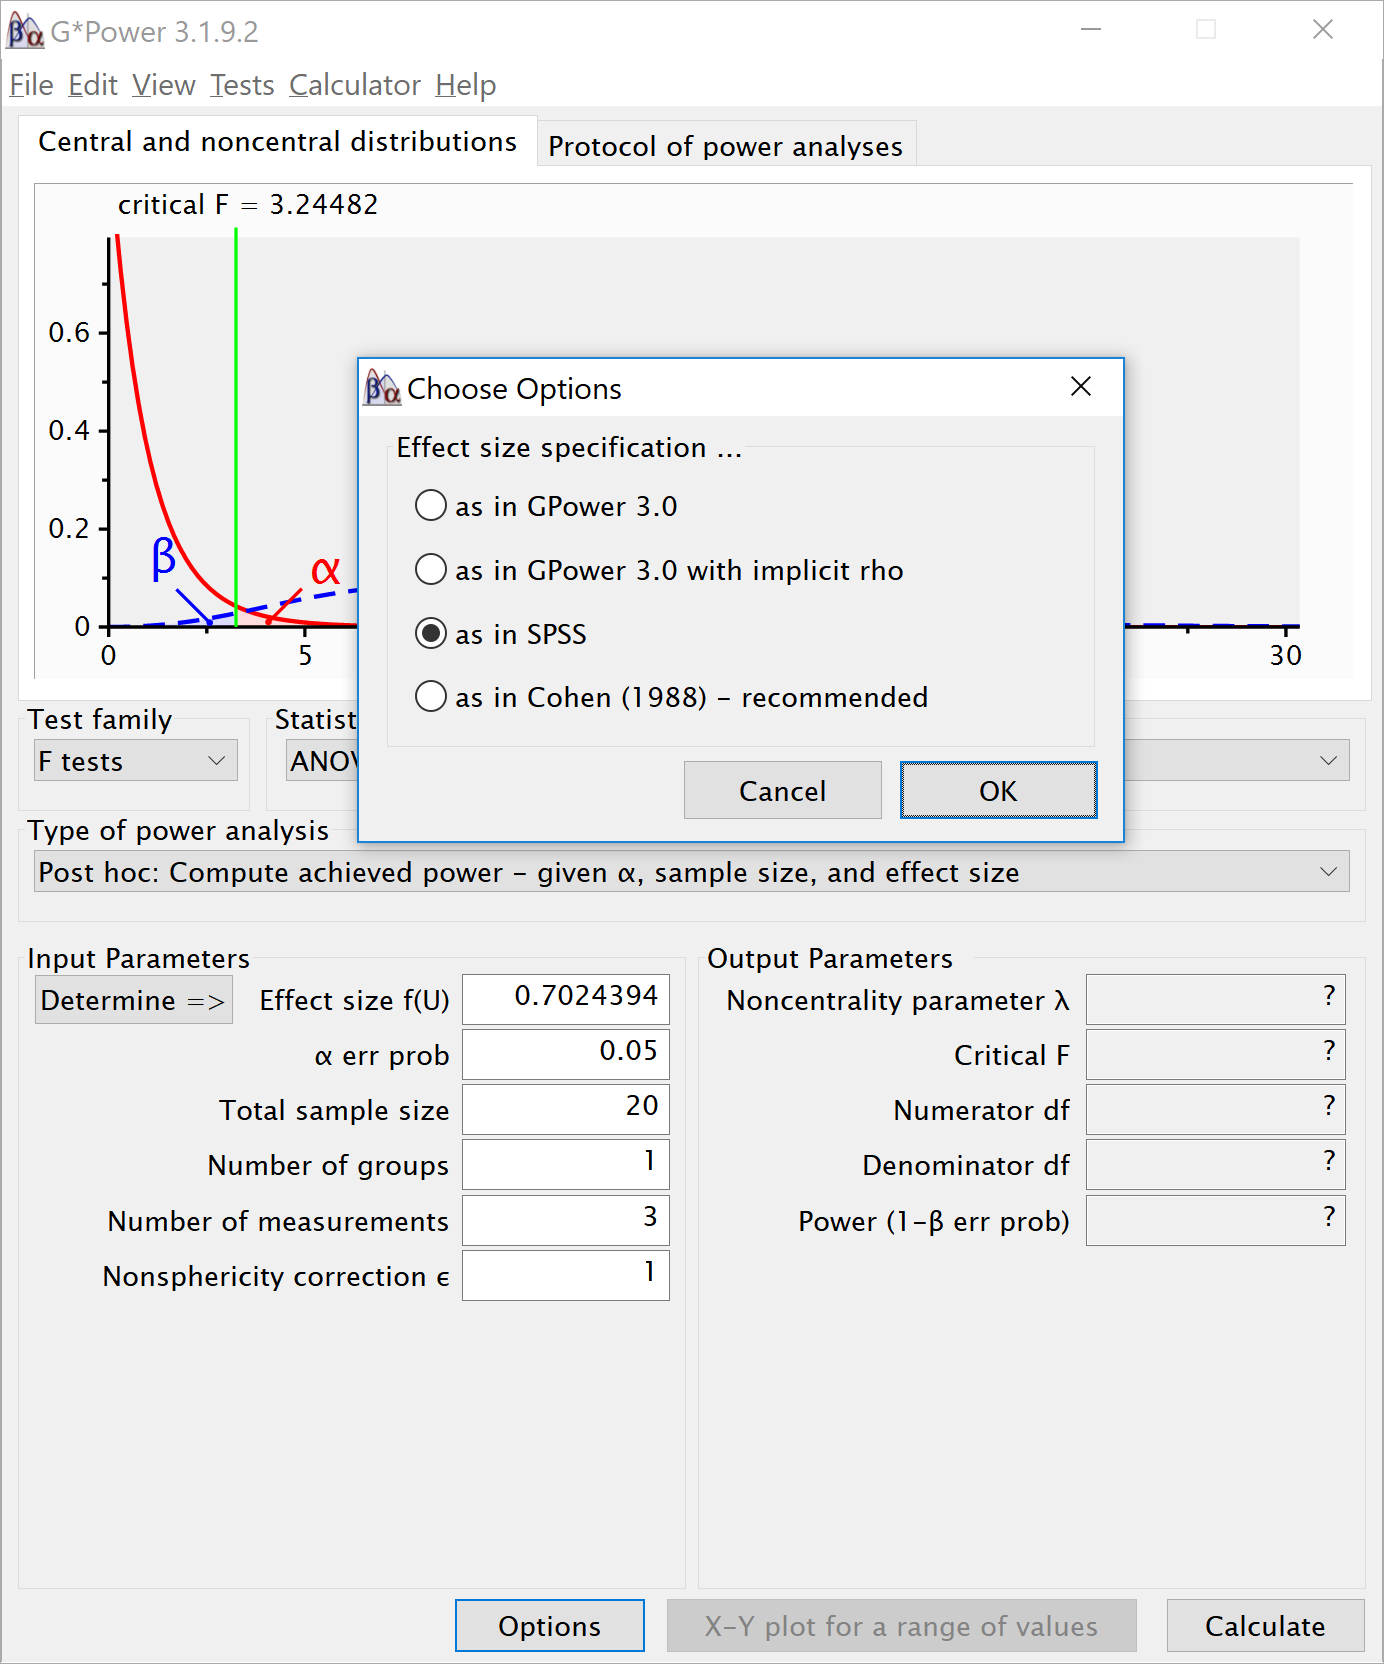
\includegraphics{screenshots/gpower_14.png}
\caption{}
\end{figure}


\end{document}
